\chapter{Τελικά Συμπεράσματα και Μελλοντικές Ε\-ξε\-λί\-ξεις} % Main chapter title
\label{chap:Chapter7}

\epigraph{”Μία επαρκής έρευνα τείνει να είναι αρκετή να υποστηρίξει τα συμπεράσματα τα οποία εξάγουμε"}{\textit{Arthur Bloch}}

Έπειτα από την ολοκλήρωση των πειραματικών διαδικασιών, είμαστε πλέον σε θέση για καταλήξουμε σε συγκεκριμένα συμπεράσματα για την παρούσα διπλωματική,
καθώς και τα σημεία τα οποία μελλοντικά μπορούν να βελτιωθούν ή να εξελιχθούν. 

\section{Συμπεράσματα}
Αρχικά, ο λόγος επιλογής της HSV μεθόδου στην συγκεκριμένη εργασία - για την υλοποίηση του object detection - ήταν διότι μπορεί να παρέχει ικανοποιητική απόδοση όντως πρώτη γενιά, με μικρές σχετικά ανάγκες επεξεργασίας. Παρόλα αυτά, κύριο αρνητικό της είναι, η ανάγκη πριν την χρήση του συστήματος να πραγματοποιηθεί calibration με βάση το scene λειτουργίας. 

Σχετικά με τα χαρακτηριστικά του Hough Transform. Αυτός είχε αποδεκτά α\-πο\-τε\-λέ\-σμα\-τα σε σκηνές με μικρό πλήθος από edges στο background. Ενώ, σε περιπτώσεις με αρκετά noisy υπόβαθρα θα πρέπει να αποφεύγεται η επιλογή του. Καθώς, ακόμα και στις δοκιμές που έγιναν σε 16-core Workstation με AMD Ryzen 7 2700X ως επεξεργαστή, παρουσιάστηκαν σημαντικά frame drops ώστε να κάνουν την ανίχνευση του αντικειμένου να μην μπορεί να γίνει σε πραγματικό χρόνο\footnote{Η συγκεκριμένη απόδοση εξαρτάται σε σημαντικό βαθμό από την επιλογή των παραμέτρων που χρησιμοποιούμε για το Hough Τransform, οι οποίες καθορίζουν και πόσο σωστά γίνεται το detection}. 

Το σύστημα δοκιμάστηκε τόσο σε indoor και outdoor περιβάλλοντα, κάτω από διαφορετικές συνθήκες φωτισμού, και ο πιο ακριβής εντοπισμός του αντικειμένου στο image plane που προέκυψε - ήταν σε κατάσταση ημέρας. Όμως, παρατηρήθηκε ότι ακόμα και σε συνθήκες χαμηλού φωτισμού ήταν δυνατή η ανίχνευση του αντικειμένου, αρκεί η πηγή φωτός να μην φωτοβολούσε υπό συγκεκριμένη κατεύθυνση, αλλά να ήταν πιο ομαλά diffused στο χώρο.

Το πιο σημαντικό συμπέρασμα από το σύνολο της εργασίας, είναι το proof of concept το οποίο μας παρέχει για την δυνατότητα εντοπισμού αντικειμένων σε real time χρόνο από low-computation low-cost Embedded Linux συστήματα. Αυτός ο εντοπισμός, έγινε με γνώμονα να αφορά drone του σμήνους για relative positioning - τα οποία φέρουν στο πλαίσιο τους παρόμοιες μορφολογίες όπως αυτό της μπάλας και για τα οποία δεν έχουμε την δυνατότητα με άλλο τρόπο να εντοπίσουμε την θέση τους (βλ. \Fig{drones-to-detect}). Παρόλα αυτά, πολύ εύκολα μπορεί να χρησιμοποιηθεί ακόμα και για τον εντοπισμό εχθρικών \Abbr{UAV}s, για τα οποία εξ' ορισμού λόγω της ετερογένειας τους δεν γνωρίζουμε την θέση τους, ακολουθώντας παρόμοια λογική ότι φέρουν ένα χαρακτηριστικό στο body τους. Ενώ, μπορεί ακόμα και να χρησιμοποιηθεί για τον προσδιορισμό της θέσης άλλων επίγειων ή εναέριων αντικειμένων από το swarm, όπως για παράδειγμα σε αποστολές \Abbr{SandR}(S\symbol{`\&}R).  

\begin{figure} [H]
	\centering
	% -----------------
    \begin{minipage}{.5\textwidth}
      \centering
      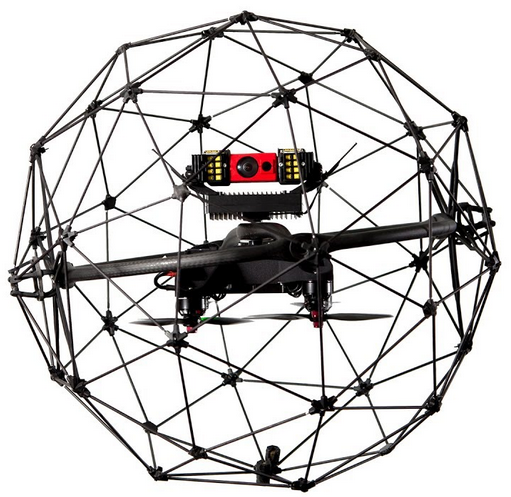
\includegraphics[width=\linewidth]{../Images/Conclusion/ball-shape-drone.png}\\
      {(a) Μορφολογία μπάλας \URI{https://www.sneakernews.top/ProductDetail.aspx?iid=369133918&pr=88.88}}
    \end{minipage}%
    % -----------------
    \begin{minipage}{.5\textwidth}
      \centering
      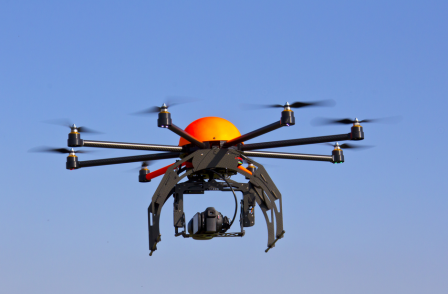
\includegraphics[width=\linewidth]{../Images/Conclusion/drone-ball-or.png}\\
      {(b) Ημισφαίριο στο πλαίσιο του \URI{https://pressgazette.co.uk/how-aerial-drones-are-becoming-latest-essential-tool-uk-news-organisations/}}
	\end{minipage}
	% -----------------
    \hfill \break
    \decoRule
    \CaptionBasedwithURL{Προτεινόμενα drone για τα οποία μπορούν να ε\-κτι\-μη\-θούν οι θέσεις} %\CaptionBasedwithURL{Possible Embedded Linux Systems} 
    \label{fig:drones-to-detect}
\end{figure}


\section{Μελλοντικές Εξελίξεις}
Μέσω των παραπάνω συμπερασμάτων, μπορούν να προταθούν και πιθανές εξελίξεις οι οποίες θα βοηθήσουν τελικά, στην πραγματοποίηση ενός συστήματος, το οποίο θα είναι σε θέση, ανεξάρτητα από το περιβάλλον και την δυναμικότητα του, να πρα\-γμα\-το\-ποιή\-σει εντοπισμό αντικειμένων στον χώρο. 

\begin{itemize}
    \item Για να ξεπεραστεί ο περιορισμός της πραγματοποίησης calibration πριν την λειτουργία του συστήματος - ακολουθώντας την ίδια προσέγγιση υ\-λο\-ποίη\-σης - μελλοντικά σημαντικό είναι η αντικατάσταση της κάμερας που χρησιμοποιήθηκε με μία Infrared (\Abbr{IR}).
    \item Επίσης, ενδιαφέρουσα μελλοντική επέκταση είναι να απομακρυνθούμε από μία αυτή καθ' αυτή computer vision προσέγγιση εντοπισμού του αντικειμένου, και να χρησιμοποιηθεί κάποια machine learning εναλλακτική. Ως παράδειγμα, χρησιμοποιώντας Tiny-YOLO για το object detection. Με αυτόν τον τρόπο θα είναι δυνατός ο εντοπισμός μεγαλύτερης γκάμας αντικειμένων από το σύστημα.
    \item Σημαντικό είναι να γίνουν μελλοντικά και συγκρίσεις του προσδιορισμού της θέσης με εναλλακτικές μεθόδους, όπως χρησιμοποιώντας Triangulation αντί για Multilateration και να αξιοποιηθεί πληροφορία σχετικά με την γωνία για το localization.
    \item Όταν το σύστημα φτάσει σε σημείο να υλοποιηθεί σε πραγματικά drones, είναι πολύ πιθανόν η κάμερα για λόγους σχετικά με τους κραδασμούς, να βρίσκεται πάνω σε Gimbal για σταθεροποίηση της εικόνας. Μία άμεση επέκταση, είναι η εκμετάλλευση του Gimbal, για λήψη μετρήσεων υπό τις βέλτιστες συ\-νθή\-κες του συστήματος - απλά κινώντας τη κάμερα ώστε το αντικείμενο παρά τα motion που πραγματοποιεί να βρίσκεται στο μέσο της εικόνας.
    \item Η ύπαρξη ενός μηχανισμού smoothing για τις μετρήσεις απόστασης και γωνίας - ώστε να αποφεύγονται τα spikes - είναι εξίσου κάτι που πρόκειται να βελτιώσει την απόδοση συνολικά του συστήματος. Καθώς έτσι, ακόμα και τις χρονικές στιγμές τις οποίες δεν ανιχνεύεται σωστά ή λόγω θορύβου περιλαμβάνει με\-γα\-λύ\-τε\-ρα σφάλματα από τα επιτρεπτά, ο προσδιορισμός της θέσης θα συνεχίζει να γίνεται σε ρεαλιστικά πλαίσια. Σε αυτό μπορεί να βοηθήσουν προσεγγίσεις με βάση το optical flow των αντικειμένων.
    \item Για να έχει πραγματική χρησιμότητα το σύστημα, ένα ακόμα ζήτημα αφορά τα ranges μέχρι τα οποία αξιόπιστα θα μπορούμε να υπολογίσουμε το αντικείμενο. Είναι σημαντικό λοιπόν να δοκιμαστούν διαφορετικές τεχνικές - πέρα από το structure from reference - για την εκτίμηση της απόσταση, με μία από αυτές ως
    προτεινόμενη να είναι το stereo vision.
    \item Σκοπός είναι να δημιουργηθεί ένα distributed αυτόνομο σύστημα το οποίο δεν θα παρουσιάζει κάποιο single point of failure σε μία πιθανή αποστολή, την οποία θα πρέπει να διεκπεραιώσει με επιτυχία. Για αυτόν τον λόγο πρέπει να βρεθεί τρόπος να ξεπεραστεί ο περιορισμός που υπάρχει μέχρι αυτήν την στιγμή και προέρχεται από την αρχιτεκτονική του ROS, ότι το master node είναι προκαθορισμένο πριν από την έναρξη λειτουργίας του συστήματος. Ενώ μελλοντικά, σε περίπτωση που το node που αναλαμβάνει αυτήν την λειτουργία του προ\-κλη\-θεί κάποιο malfunction θα πρέπει να μπορεί on the fly να αντικατασταθεί και να αναλάβει κάποιο άλλο drone αυτήν την αρμοδιότητα.
    \item Πρέπει επιπλέον να γίνουν δοκιμές με πραγματικά δεδομένα για τις θέσεις των nodes, τα οποία με μεγάλη ακρίβεια θα προσδιορίζουν την θέση τους. Αυτό μπορεί να γίνει είτε με χρήση RTK GPS είτε με οικονομικότερες εναλλακτικές αν συνεχίζει να μας ενδιαφέρει το relative positioning. Μία εξ' αυτών είναι η χρήση των UWB για το σχετικό localization πρώτα των drones μεταξύ τους - με τρόπους που περιγράφτηκαν στο κεφάλαιο με το θεωρητικό υπόβαθρο - και σε δεύτερο επίπεδο, γνωρίζοντας τις σχετικές θέσεις τελικά να πρα\-γμα\-το\-ποιού\-με τον εντοπισμό ετερογενούς object. 
    \item Σχετικά με τον καθορισμό του ID, μπορούν να επιλεχθούν τεχνικές κω\-δι\-κο\-ποί\-η\-σης για τον καθορισμό τους, ώστε σε πεπερασμένο χρονικό διάστημα να γνωρίζουμε σε ποιο node αναφερόμαστε. Δύο πιθανές προσεγγίσεις είναι με χρήση Huffman ή Golomb codes.
    \item Η πιο σημαντική μελλοντική επέκταση, είναι φυσικά οι δοκιμές του συστήματος σε πραγματικά drone, και πιθανόν να βρεθεί τρόπος να αντικατασταθεί η ανάγκη για επικοινωνία μέσω WiFi με μία που να μπορεί να καλύψει αξιόπιστα μεγαλύτερες αποστάσεις.
  \end{itemize}



